\chapter{Fazit}
Durch die generalisierte Lösung auf Basis eines abstrakten Packages 'BaseSwarm', das allen realisierten Algorithmen zugrunde liegt konnte mit der Realisierung der Bibliothek zu modernen Algorithmen aus dem Kontext der Schwarmintelligenz eine sehr gute Basis geschaffen werden, um sowohl die drei gefoderten Algorithmen 'Grey Wolf Optimization', 'Rat Swarm Optimization' und 'Elephant Herding Optimization' in Lehre und Forschung einsetzen zu können, als auch auf der Basis des 'BaseSwarm' weitere Algorithmen auf diesem Fundament einfach implementieren zu können (vgl. \autoref{uml_img}). \\
Auf Basis der Ackleyfunktion konnten die realisierten Algorithmen gegenübergestellt werden und im direkten Vergleich gegeneinander auf gleicher Hardware Funktion und Geschwindigkeit pro Algorithmus sichergestellt werden. Dazu sind die jeweiligen Testläufe, inkl. Zeitmessung in \autoref{test_eho} (Elephant Herding Optimization), \autoref{test_rso} (Rat Swarm Optimization) und \autoref{test_gwo} (Grey Wolf Optimization) zu finden.

\begin{figure}[ht]
    \begin{center}
        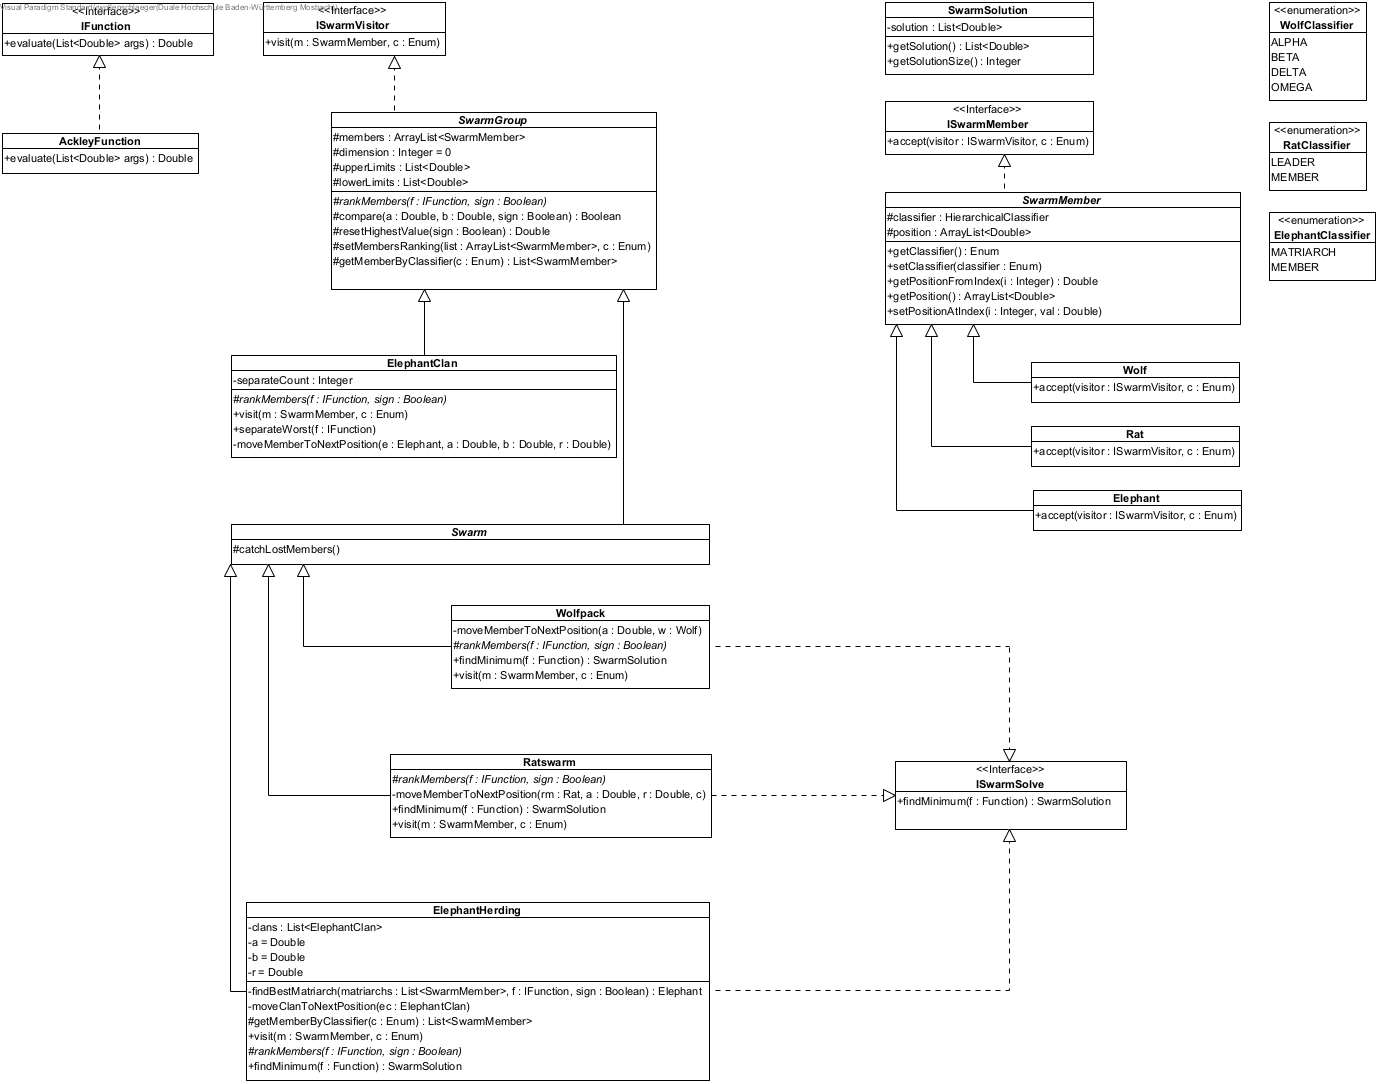
\includegraphics[width=1.0\textwidth]{../SwarmOptimization.jpg}
        \caption{UML Bibliothek Schwarmintelligenz}
        \label{uml_img}
    \end{center}
\end{figure} 

\begin{figure}[ht]
    \begin{center}
        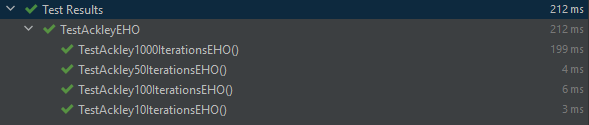
\includegraphics[width=.7\textwidth]{./assets/img/Test_eho.PNG}
        \caption{Testergebnisse Elephant Herding Optimization}
        \label{test_eho}
    \end{center}
\end{figure}
\begin{figure}[ht]
    \begin{center}
        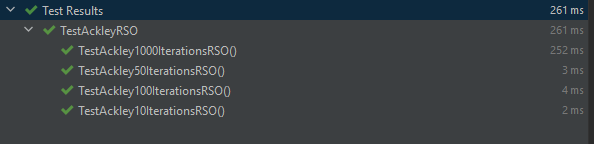
\includegraphics[width=.7\textwidth]{./assets/img/Test_rso.PNG}
        \caption{Testergebnisse Rat Swarm Optimization} 
        \label{test_rso}
    \end{center}
\end{figure}
\begin{figure}[ht]
    \begin{center}
        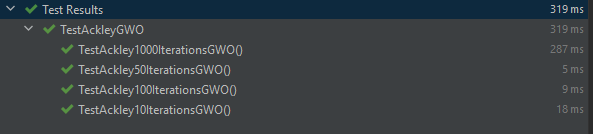
\includegraphics[width=.7\textwidth]{./assets/img/Test_gwo.PNG}
        \caption{Testergebnisse Grey Wolf Optimization}
        \label{test_gwo}
    \end{center}
\end{figure}
